\documentclass{article}
\usepackage{amsmath, amsthm, amssymb}
\usepackage{makeidx}
\usepackage{amsbsy}
\usepackage{graphicx}
\usepackage{bm}
\usepackage{color}
\textwidth=6.2in
\textheight=9.0in
\oddsidemargin=0.0in
\evensidemargin=0.0in

\begin{document}
\def\theequation{\arabic{section}.\arabic{equation}}
\setcounter{page}{1}
\newcommand{\bb}{\boldsymbol{\beta}}
\newcommand{\bh}{\boldsymbol{\hat{\beta}}}
\newcommand{\by}{\widetilde{\boldsymbol{y}}}
\newcommand{\Y}{\widetilde{\boldsymbol{Y}}}
\newcommand{\bX}{\widetilde{\boldsymbol{X}}}
\newcommand{\be}{\boldsymbol{\widetilde{\epsilon}}}
\newcommand{\0}{\boldsymbol{0}}
\newcommand{\bth}{\boldsymbol{\hat{\theta}}}
\newcommand{\bt}{\boldsymbol{\theta}}
\newcommand{\bT}{\boldsymbol{T}}
\newcommand{\bF}{\boldsymbol{F}}
\newcommand{\D}{\boldsymbol{D}}
\newcommand{\bR}{\boldsymbol{R}}
\newcommand{\br}{\boldsymbol{r}}
\newcommand{\bS}{\boldsymbol{S}}
\newcommand{\bM}{\boldsymbol{M}}
\newcommand{\bN}{\boldsymbol{N}}
\newcommand{\bI}{\boldsymbol{I}}
\newcommand{\V}{\boldsymbol{V}}
\newcommand{\K}{\boldsymbol{K}}
\newcommand{\VD}{\boldsymbol{V_D}}
\newcommand{\bD}{\boldsymbol{\hat{b}}_{\boldsymbol{D}}}
\newcommand{\bRD}{\boldsymbol{\hat{b}}_{\boldsymbol{RD}}}
\newcommand{\bGD}{\boldsymbol{\hat{b}}_{G\boldsymbol{D}}}
\newcommand{\bGRD}{\boldsymbol{\hat{b}}_{G\boldsymbol{RD}}}
\newcommand{\CD}{\boldsymbol{C_D}}
\newcommand{\MD}{\boldsymbol{M_D}}
\newcommand{\ND}{\boldsymbol{N_D}}
\newcommand{\Q}{\boldsymbol{Q}}
\newcommand{\ba}{\boldsymbol{a}}
\newcommand{\bY}{\boldsymbol{Y}}
\newcommand{\bx}{\boldsymbol{x}}
\newcommand{\bA}{\boldsymbol{A}}
\newcommand{\bG}{\boldsymbol{G}}
\newcommand{\bC}{\boldsymbol{C}}
\newcommand{\bH}{\boldsymbol{H}}
\newcommand{\bP}{\boldsymbol{P}}
\newcommand{\bs}{\sigma}
\newcommand{\bet}{\boldsymbol{\eta}}
\newcommand{\bPh}{\boldsymbol{\Phi}}
\newcommand{\bd}{\boldsymbol{\delta}}
\newcommand{\W}{\mathcal{W}}
\newcommand{\A}{\mathcal{A}}
\newcommand{\B}{\mathcal{B}}
\newcommand{\E}{\mathcal{E}}
\newcommand{\N}{\mathcal{N}}
%\newcommand{\D}{\mathcal{\boldsymbol{D}}}
\newcommand{\beq}{\begin{eqnarray}}
\newcommand{\eeq}{\end{eqnarray}}
\newtheorem{thm}{Theorem}[section]
\newtheorem{cor}{Corollary}[section]
\newtheorem{lem}{Lemma}[section]
\newtheorem{rem}{Remark}[section]
\newtheorem{prop}{Proposition}[section]
	
\title{\bf{Liu-type estimators for the Elliptical SUR Model}}
\author{Morteza Amini$^1$\footnote{Corresponding Author ({\em Email: morteza.amini@ut.ac.ir})} Mohammad Arashi$^2$, and Mahdi Roozbeh$^3$\\
\small{$^{1}$ Department of Statistics, School of Mathematics, Statistics, and Computer Science,}\\
\small{College of Science, University of Tehran, Iran}\\
\small{$^{2}$ Department of Statistics, Faculty of Mathematical Sciences,}\\
\small{Ferdowsi University of Mashhad, P. O. Box 1159, Mashhad 91775, Iran.}\\
\small{$^{3}$ Department of Statistics, Faculty of Mathematics, Statistics and Computer Sciences,}\\
\small{Semnan University, Iran}
}

\date{}
\maketitle
	
\begin{quotation}
\noindent {\it \textbf{Abstract:}}
This paper investigates the application of Liu estimators within the seemingly unrelated regression (SUR) model under conditions of multicollinearity and elliptically distributed errors—an issue often observed in applied economic research. The conventional SUR setup is generalized by incorporating partially linear components, which improves adaptability for intricate econometric specifications. Asymptotic characteristics of the introduced estimators are established, alongside detailed risk assessments that highlight their theoretical benefits. A wide range of Monte Carlo experiments confirms the enhanced effectiveness of this estimator relative to traditional approaches.
\end{quotation}\par
\noindent {\it  \textbf{Keywords}}: Elliptical errors; Multicollinearity; Partially linear model; Seemingly unrelated regression.
	
\section{Introduction}
Shrinkage methods serve as an effective strategy in statistics, particularly for addressing multicollinearity and enhancing the accuracy of estimations. Well-known techniques such as ridge regression (RE) and Stein-type estimators (SE) have been introduced to resolve multicollinearity issues within regression frameworks. These approaches constrain coefficient magnitude through penalization, thereby lowering variance and frequently boosting predictive capability. Nevertheless, shrinkage estimators are not without practical difficulties. Careful attention to model specification is required, since computational demands can become significant in intricate scenarios, and violations of key assumptions may weaken their performance. Additionally, multicollinearity continues to pose a serious problem by inflating standard error estimates, compromising inferential validity, and causing misleading interpretations regarding the relevance of individual predictors. Consequently, there is a clear need for robust and properly tuned estimation methods—like contemporary shrinkage techniques—that explicitly incorporate these concerns while preserving computational tractability and clarity of interpretation. For relevant literature, see \cite{Månsson2012-2}, \cite{Månsson2012-3}, \cite{Månsson2013}, \cite{Algamal2018}, \cite{Qasim2019}, \cite{Qasim2020}, \cite{Amin2021}, \cite{Algamal2022} among others.

The seemingly unrelated regression (SUR) model, originally proposed by \cite{Zellner1962}, comprises several regression equations whose error terms are correlated, even if the equations themselves seem independent at first glance. This cross-equation error correlation allows the SUR approach to combine information across equations, thereby yielding estimates that are more efficient compared to applying ordinary least squares separately to each equation. An additional application of SUR is in analyzing a single household's demand across various goods. In that context, however, theoretical economic principles introduce constraints linking the equations—such as those arising from budget limitations—which need to be integrated directly into the estimation procedure.
	
Despite the frequent use of the elliptical distribution in SUR modeling, the design of shrinkage estimators under this assumption has received little attention. Given the distinctive features of this distributional framework within econometric SUR applications, we intend to introduce shrinkage-based techniques for parameter estimation in the presence of multicollinearity. For recent advances in related shrinkage estimation approaches, see \cite{Saleh2022} and the references cited therein.

 We introduce the first Liu-style shrinkage estimator designed for partially linear Seemingly Unrelated Regression (SUR) models, which integrates structured penalization with adaptable nonparametric elements. This approach connects classical multivariate regression with contemporary regularization theory, addressing a significant gap in the literature. A fully data-dependent and theoretically grounded method is developed to determine the Liu shrinkage parameter via Cross-Validation, removing reliance on arbitrary tuning or costly repeated cross-validation procedures.

The organization of this paper proceeds as follows. In Section 2, we provide a formal specification of the seemingly unrelated regression (SUR) model with elliptically distributed errors and investigate the asymptotic behavior of the weighted least squares estimator for parameter testing. Section 3 then constructs shrinkage estimators using a unified linear estimation framework and derives their large-sample properties to assess theoretical behavior. Finally, Section 4 offers an extensive comparison of these estimators based on risk dominance metrics.
	
\setcounter{equation}{0}
\section{The SUR Model}
Following the notation established by \cite{Roozbeh2012}, this section outlines the model and provides essential background results concerning least squares estimation in partially linear SUR systems. Let the system consist of $M$ equations
\begin{eqnarray*}
\bY_i=\boldsymbol X_i\bb_i+\boldsymbol f_i(\boldsymbol t)+\boldsymbol{\epsilon}_i, \;i=1,...,M,	
\end{eqnarray*}
where $\bY_i$ is a vector of $n\times1$ responses, $\boldsymbol X_i=(\bx_1,\ldots,\bx_n)^\top$ is a $n\times p_i$ fixed design with rank $p_i$ on the explanatory variables $\bx_j\in\mathbb{R}^{p_i}$, $j=1,\ldots, n$, $\bb_i$ is a
$p_i\times1$ vector of regression coefficients, $\boldsymbol{f}_i(\boldsymbol t)$ is a $n\times1$ vector of
nonparametric functions and $\boldsymbol{\epsilon}_i$ is a
$n\times1$ vector of random errors, with ${\mathbb{E}}(\boldsymbol\epsilon_i\boldsymbol\epsilon^\top_j)=v_{ij}\bI_n$, where $v_{ij}$ designate the covariance between the $i^{th}$ and $j^{th}$ equations for each observation in the sample. Here, $M$ is the number of equations in the system, $n$ is the number of observations per equation and $p_i$ is the number of rows in the vector $\bb_i$.
Assume $\bY=(\bY^\top_1,\bY^\top_2, \ldots, \bY^\top_M)^\top$, $\boldsymbol X={\rm Diag}(\boldsymbol X_1,\boldsymbol X_2, \ldots, \boldsymbol X_M)$, $\bb=(\bb^\top_1,\bb^\top_2, \ldots, \bb^\top_M)^\top$,
$\boldsymbol f(\boldsymbol t)=\big(\boldsymbol f^\top_1(\boldsymbol t), \boldsymbol f^\top_2(\boldsymbol t),\ldots, \boldsymbol f^\top_M(\boldsymbol t)\big)^\top$ and $\boldsymbol{\epsilon}=(\boldsymbol{\epsilon}^\top_1,\boldsymbol{\epsilon}^\top_2, \ldots, \boldsymbol{\epsilon}^\top_M)^\top$. Then the $M$ equations can be integrated into the following form
\begin{equation}\label{eq21}
\boldsymbol{Y}=\boldsymbol{X}\bb+\boldsymbol{f}(\boldsymbol t)+\boldsymbol{\epsilon},
\end{equation}
where $\bY,~\boldsymbol{f}(\boldsymbol t)$ and $\boldsymbol{\epsilon}$ are each of dimension $nM\times1$, $\boldsymbol{X}$ is of dimension $nM\times p$,
$p=\sum_{i=1}^Mp_i$, and $\bb$ is a vector of $p\times1$ parameters. Furthermore,
${\mathbb{E}}(\boldsymbol{\epsilon})=\0$, and ${\mathbb{E}}(\boldsymbol{\epsilon}\boldsymbol{\epsilon^\top})=\V$, with
$\V_{ij}=v_{ij}\bI_n,
$
as an $nM\times nM$ positive definite symmetric matrix, or simply as $(v_{ij})\otimes\bI_n$, where $\otimes$ represents the Kronecker product. This assumption enforces homoscedasticity between the errors and not autocorrelation. However, it is assumed that there is a contemporaneous correlation between corresponding errors in different equations.
	
For the estimation of $\bb$, we use the partial kernel smoothing estimator and thus, using \cite{Speckman1988}, we estimate $f_i(\cdot)$ via
\begin{eqnarray*}
\hat{f}_i(t_j,\bb_i)=\sum_{k=1}^n W_{n_k}(t_j)(y_{ik}-\bm{x}^\top_{ik}\bb_i),
\end{eqnarray*}
where the positive weight functions $W_{n_k}(\cdot)$ satisfy $\max\sum_{j=1}^n W_{n_k}(t_j)=O(1)$, $\max W_{n_k}(t_j)=O(n^{-2/3})$, and $\max\sum_{k=1}^nW_{n_k}(z_j)I(|t_i -t_j|>c_n)=O(d_n)$, for some sequences $c_n$ and $d_n$ satisfying $\lim\sup nc_n^3<\infty$, and $\lim\sup nd_n^3<\infty$.
Now, define
\begin{eqnarray*}
\bC &=& \bX^\top\V^{-1}\bX = {\rm Diag}(\bC_{1},\ldots, \bC_{M}), \quad \bC_{i}=\bX^\top_i\V_{ii}^{-1}\bX_i, \\
\Y &=& (\widetilde{y}_{11},\ldots, \widetilde{y}_{1n},\widetilde{y}_{21}, \ldots, \widetilde{y}_{2n},\ldots, \widetilde{y}_{M1},\ldots, \widetilde{y}_{Mn})^\top, \\
\bX &=& (\widetilde{\bx}_{11},\ldots, \widetilde{\bx}_{1n},\widetilde{\bx}_{21},\ldots, \widetilde{\bx}_{2n},\ldots, \widetilde{\bx}_{M1},\ldots, \widetilde{\bx}_{Mn})^\top, \\
\widetilde{y}_{ij} &=& y_{ij}-\sum_{j=1}^{nM} W_{n_j}(t_i)y_{ij}, \;\;
\widetilde{\bx}_{ij} = \boldsymbol{x}_{ij}-\sum_{j=1}^{nM} W_{n_j}(t_i)\boldsymbol{x}_{ij}, \quad i=1,\ldots, M,\; j=1,\ldots, n.
\end{eqnarray*}

To estimate $\bb$, we minimize the least squares criterion.
\[
SS(\bb)=(\Y-\bX\bb)^\top\V^{-1}(\Y-\bX\bb)
\]
to get the weighted least square estimator (WLSE) given by
\begin{equation}\label{eq24}
\bh^{SUS} = \bC^{-1}\bX^\top\V^{-1}\Y.
\end{equation}
To expand and improve the flexibility of our modeling framework, we assume that the random error terms are drawn from a multivariate elliptical distribution.
	
Suppose now that $\boldsymbol{\epsilon}$ follows a distribution belonging to the family of elliptically contoured distributions (ECDs), denoted by $E_{nM}(\0,\V,\psi)$, whose characteristic function takes the form
$\phi_{\boldsymbol{\epsilon}}(\boldsymbol{t}) = \psi\left(\boldsymbol{t}^\top\V\boldsymbol{t}\right)$,
where $\psi : [0,\infty)\rightarrow\mathbb{R}^+$ acts as the characteristic generator. Assuming a density exists, it can be expressed as
\begin{equation}
f(\boldsymbol{\epsilon}) \propto |\V|^{-\frac{1}{2}}g\left(\boldsymbol{\epsilon}^\top\V^{-1}\boldsymbol{\epsilon}\right),
\end{equation}
with $g(.)$ a non-negative function on $\mathbb{R}^+$ ensuring that $f(.)$ is a valid density relative to a $\sigma$-finite measure $\mu$ on $\mathbb{R}^{nM}$. In such a setting, one would typically write $\boldsymbol{\epsilon}\sim E_{nM}(\0,\V,g)$.

Following \cite{Galea2000}, let $m_o$ denote the maximum of $g(\cdot)$. For the normal and Student's t-distributions, $m_o$ equals $nM$. In the case of the power exponential distribution, $m_o = (nM/\alpha)^{1/\alpha}$, where $\alpha$ is the power parameter. For distributions such as the contaminated normal or logistic, $m_o$ must be computed numerically. Specifically for the logistic distribution, the relation is given by
$\frac{nM}{2m_o} = \tanh\left(\frac{m_o}{2}\right).$

We compare our proposed method with the classical SUR estimator of \cite{Zellner1962}, which continues to serve as the reference standard for multi-equation systems featuring correlated disturbances. Although Zellner's estimator is efficient when the model is correctly specified, it becomes unreliable under multicollinearity among the regressors, resulting in inflated variances and misleading inference—a shortcoming that our shrinkage procedure directly tackles. We further consider ridge-type SUR estimators, including those introduced by \cite{Liu2014}, which adapt ridge regression to the SUR setting through the addition of an $l_2$ penalty applied to the coefficient vector of each equation. While these methods are effective at variance reduction, they typically shrink coefficients either equation by equation or impose diagonal penalty matrices, thus not fully utilizing the off-diagonal components of the error covariance matrix. By contrast, our Liu-type estimator integrates shrinkage directly into the joint SUR likelihood, preserving the complete covariance structure and providing more coherent regularization across equations. A key distinction of our approach is that, unlike many existing shrinkage methods, the Liu-type estimator retains the original SUR error covariance structure throughout the regularization process. This feature allows cross-equation information to be exploited fully, ensuring that the resulting estimates remain aligned with the underlying economic or structural relationships. Furthermore, the scalar shrinkage parameters $d_i$ are analytically manageable, making selection straightforward through cross-validation (CV) and reducing sensitivity to misspecification of the cross-equation correlations.
	
\setcounter{equation}{0}
\section{Linear Unified Estimators}
It is important to note that the properties of the weighted least squares estimator (WLSE) of $\bb$ are strongly influenced by the characteristics of the information matrix $\bC$. When $\bC$ is ill-conditioned, the WLSE exhibits excessively large sampling variances. Consequently, some regression coefficients may become statistically insignificant or carry incorrect signs, making reliable inference challenging for the researcher. As a remedy, \cite{Roozbeh2012} introduced the ridge-weighted least squares estimator (RWLSE). As a shrinkage technique, the RWLSE is often regarded as a standard solution to multicollinearity. However, when the ill-conditioning is severe, a small ridge parameter proves insufficient. Conversely, large ridge parameter values introduce substantial bias into the estimates. Inspired by \cite{Liu1993} and \cite{Akdeniz1995}, we instead seek a regularization parameter matrix $\bT_{\D}$ such that $\bT_{\D}\hat{\bb}^{\rm SUS}$ is close to $\bb$, thereby focusing on penalizing the magnitude of $(\bT_{\D}\hat{\bb}^{\rm SUS}-\bb)$ rather than $\bb$ itself, as is done in the RWLSE.
	
Thus, we propose the following linear unified (Liu, refer to \cite{Akdeniz1995} and \cite{Liu1993}) weighted least square estimator (LWLSE)
\begin{eqnarray}
\bh^{\rm SUS}(\D) = \bT_{\D}\bh^{\rm SUS},
\end{eqnarray}
where $\bT_{\D}=(\bC+\bI_p)^{-1}(\bC+\boldsymbol{D})$, $\D={\rm Diag}(\D_1,\D_2,...,\D_M)$, $\D_i=d_i\bI_{p_i}, 0\leq d_i\leq1$ are the shrinking parameters for $i=1,..,M$, and $p=\sum_{i=1}^Mp_i$.
	
Let $\bC_{\D}=\bT_{\D}\bC^{-1}\bT_{\D}$. In an asymptotic sense, for the shrinkage methodologies, it is easy to see
\begin{eqnarray}
\sqrt{nM}(\bh^{\rm SUS}(\D)-\bb) &\overset{\mathcal{D}}{\to}& N_p\left((\bT_{\D}-\bI_p)\bb,\bC_{\D}\right),
\end{eqnarray}
	
The bias of the proposed estimators is routinely derived from Saleh (2006) and Hassanzadeh Bashtian et al. (2011). Therefore, we omit all derivations. The asymptotic distributional biases of all Liu machine learners are given by
\begin{eqnarray*}
{\rm Bias}(\bh^{\rm SUS}(\D)) &=& - (\bI_p - \D)(\bC + \bI_p)^{-1}\bb.
\end{eqnarray*}
	
The asymptotic distributional risks of all Liu machine learners are given by
\begin{eqnarray*}
{\rm Risk}(\bh^{\rm SUS}(\D)) &=& {\rm tr}(\bT_{\D}^\top\bC^{-1}\bT_{\D}) + \bb^\top(\bC + \bI_p)^{-1}(\bI_p - \D)^2(\bC + \bI_p)^{-1}\bb.
\end{eqnarray*}

\setcounter{equation}{0}
\section{ Numerical Experiments}

In this section, we present the results of several numerical experiments designed to illustrate the benefits of the proposed methodologies within partially linear SUR models. For this purpose, we evaluate the performance of our approaches through Monte Carlo simulation studies, along with an application to a real-world dataset based on Grunfeld's investment data.

\subsection{Simulation study}

In this section, we proceed to compare the proposed estimators through numerical computations. To evaluate the proposed estimators with respect to the shrinkage parameter $d$, we compare the risk functions of the Liu-type versions of the estimators with their non-Liu-type counterparts, and define the scalar ${\delta}$ as follows:
\begin{eqnarray}\label{eq52}
\delta={\rm Risk}(\bh^{{\rm PR}~or~{\rm R}~or~{\rm U}})-
{\rm Risk}(\bh^{{\rm PR}~or~{\rm R}~or~{\rm U}}(\D)).
\end{eqnarray}
\begin{figure}
\centerline{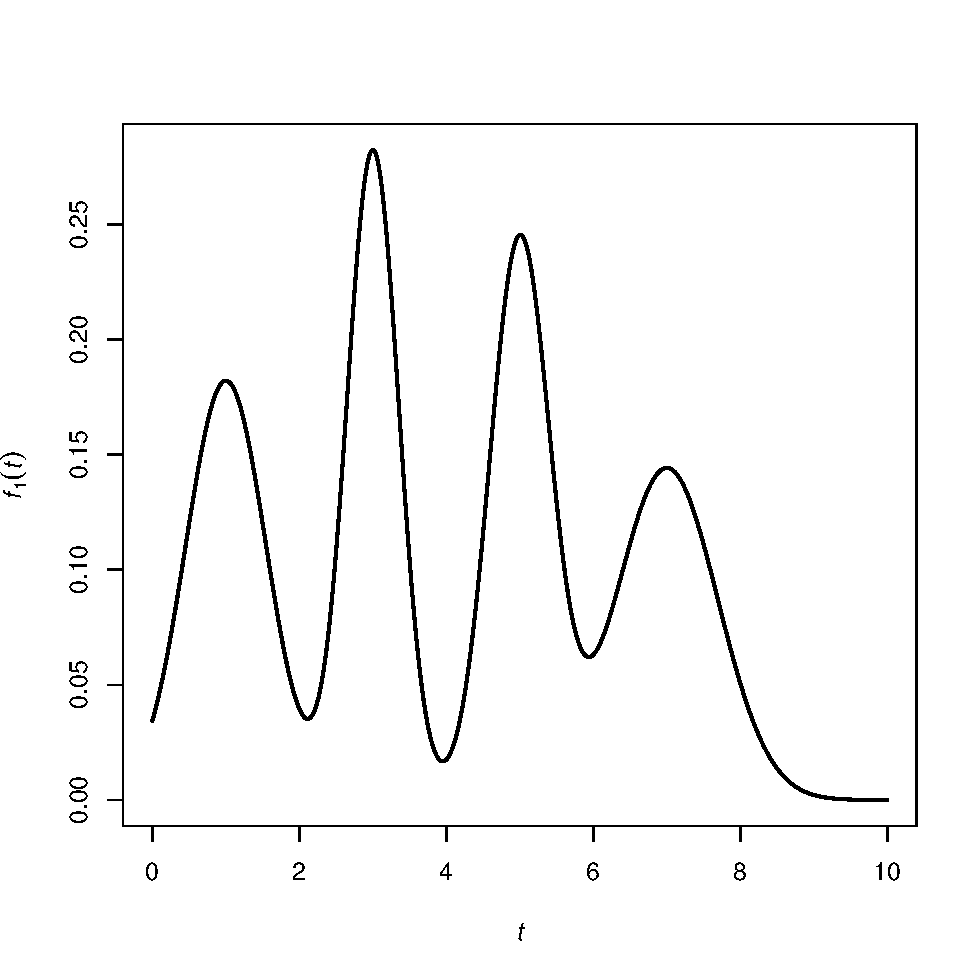
\includegraphics[scale=.25]{f1-eps-converted-to.pdf} 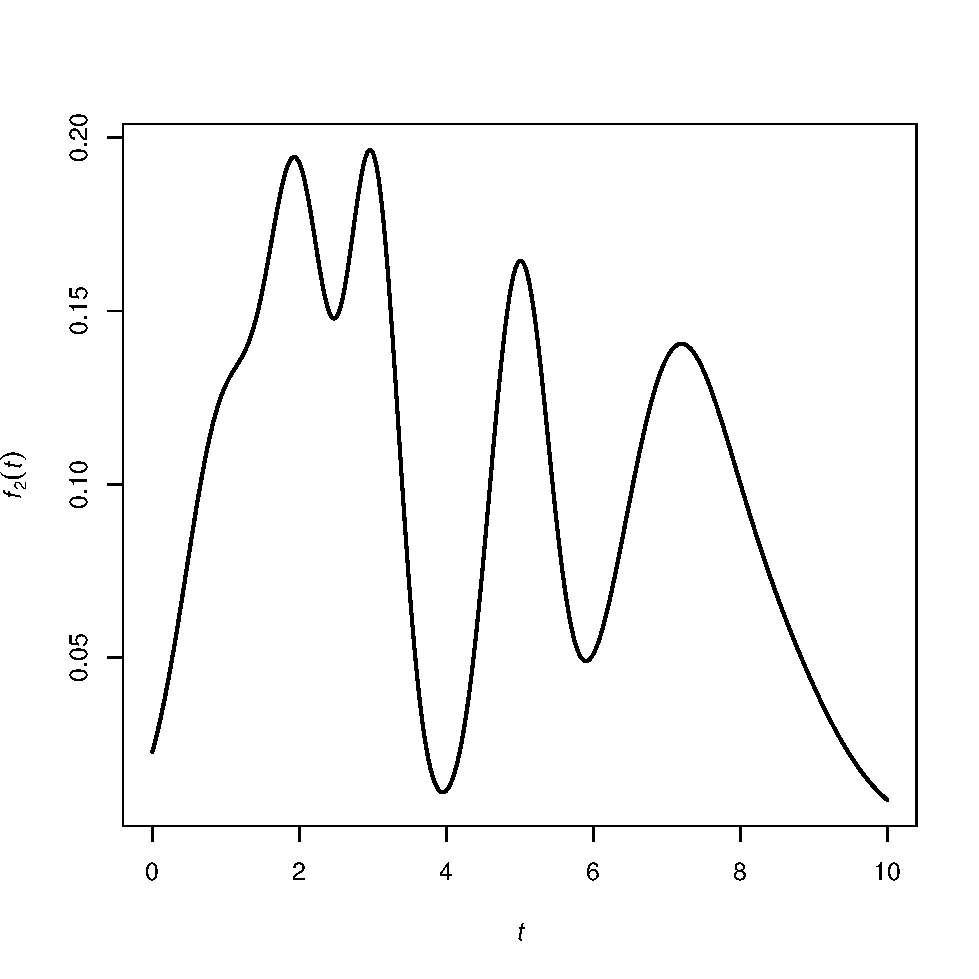
\includegraphics[scale=.25]{f2-eps-converted-to.pdf} 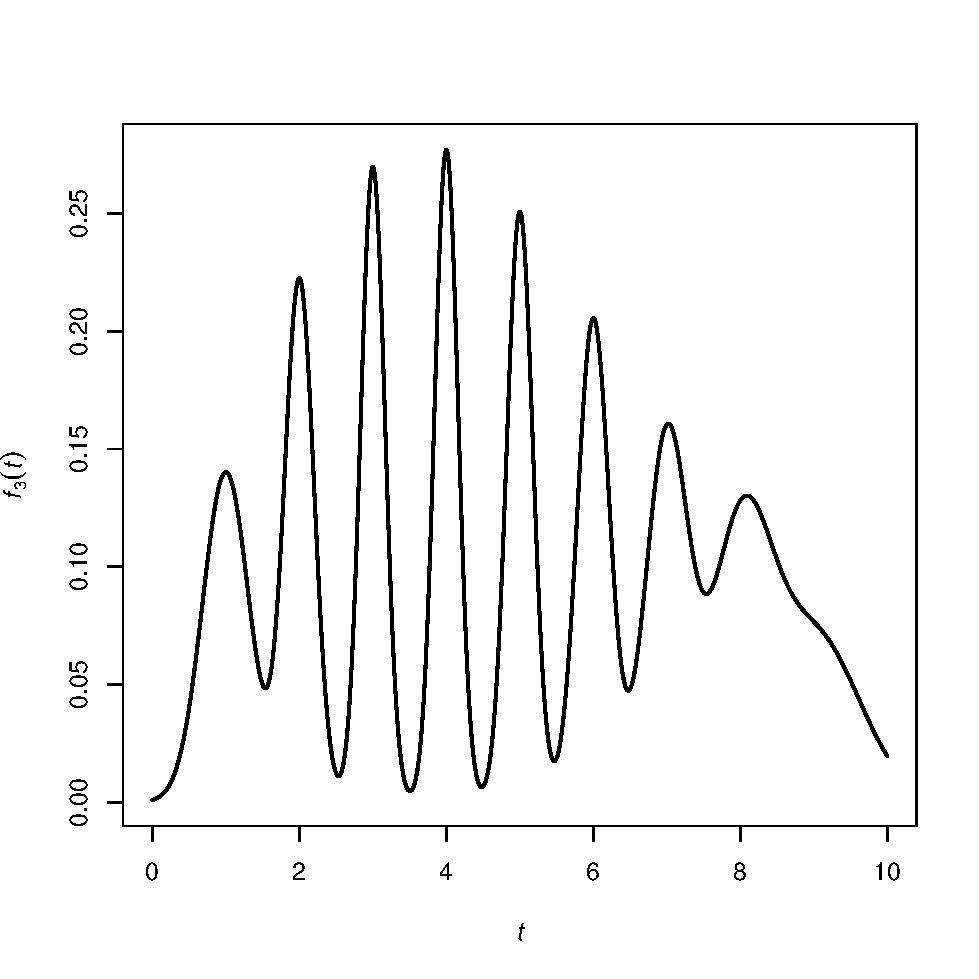
\includegraphics[scale=.25]{f3-eps-converted-to.pdf}}
%\caption{\small{The diagrams of the nonparametric functions under study.}}
%\label{fig1}
\end{figure}
In this study we simulate the response for $M=3$ equations and $T=100$ with $10^4$ iterations from the
model \eqref{eq21}, with 
 $\bb_1=(1,2,3,-1,5), \bb_2=(-1,-2,-3,1,-5), \bb_3=(-1.5,2,-3,1,2)$, for
$i=1,\ldots,T,~$${\bx}_i\thicksim N_5(\boldsymbol{\mu}_x,\boldsymbol{\Sigma}_{{x}})$
with
$$\boldsymbol{\mu_x}=\left(-17.5,19,-19,-18,-8,\right)^\top,
~\boldsymbol{\Sigma_{{x}}}= r_x \mathbf{1}_5 + (1- r_x) \mathbf{I}_5,$$
where $r_x=0.75$, $\boldsymbol{\epsilon}\thicksim
N_{TM}(\0,\boldsymbol{V})~$
and
\begin{eqnarray*}
&&\boldsymbol\epsilon\thicksim {Mt}_n(\0,\sigma^2\V_1,10),~\sigma^2=0.64,~(\V_1)_{ij}=\exp\big(-|i-j|\big),~i,j=1,\ldots,n,
\end{eqnarray*}
in which ${Mt}_n(\boldsymbol\delta,\boldsymbol\Sigma,\nu)$  denotes the n-variate noncentral t-distribution with non centrality parameter of $\delta$, scale matrix of $\boldsymbol\Sigma$ and $\nu$ degrees of freedom. It is worth noting that the multivariate t-distribution is an important distribution in the class of elliptically contoured distributions and plays an important role in robust statistical inference, particularly for heavy
tailed distributions involving outliers and extreme values.	
We consider the following three functions as nonparametric parts:
\begin{eqnarray*}
f_1(t_i)&=&\frac{1}{4}\sum_{j=1,j\neq2,4,6}^{7}\phi\Big(t_i;j,\big((j+2)/10\big)^j\Big),
\quad
f_2(t_i)=\frac{1}{6}\sum_{j=1,j\neq4,6}^{8}\phi\Big(t_i;j,\big((j+2)/10\big)^j\Big)\\
f_3(t_i)&=&\frac{1}{9}\sum_{j=1}^{9}\phi\big(t_i;j,(j/10)^j\big),
\end{eqnarray*}
which are mixtures of normals and $\phi(x;\mu,\sigma^2)$ is a normal density function with mean $\mu$ and variance $\sigma^2$ for $t_i=10i/n~$.

\begin{figure}
\centerline{
\includegraphics[scale=.2]{riskULEg099-eps-converted-to.pdf} 
\includegraphics[scale=.2]{riskRLEg099-eps-converted-to.pdf}
\includegraphics[scale=.2]{deltaULEg099-eps-converted-to.pdf}
\includegraphics[scale=.2]{deltaRLEg099-eps-converted-to.pdf}}
\caption{\small{The diagram of risks of (from left to right) ULE and RLE, and $\delta$ differences of the ULE and RLE versus $d$.}}\label{fig6}
\end{figure}


For the weight function $W_{n_i}(t_j)$, we use
\begin{equation*}
W_{n_i}(t_j)=\frac{1}{nMh_{nM}}K\Big(\frac{t_i-tj}{h_{nM}}\Big)=\frac{1}{nMh_{nM}}.\frac{1}{\sqrt{2\pi}}\exp\Big\{-\frac{(t_i-t_j)^2}{2h_{nM}^2}\Big\},
~h_{nM}=0.01,
\end{equation*}
which is Priestley and Chao's weight with the Gaussian kernel. We
also apply the cross-validation (CV) method to select the
optimal bandwidth $h_{nM}$, which minimizes the following CV function
\begin{equation*}
CV(h_{nM})=\frac{1}{nM}\sum_{i=1}^{nM}\Big(\Y^{(-i)}-\bX^{(-i)}\bh^{*^{(-i)SUS}}(\D)\Big)^2,
\end{equation*}
where $\bh^{*^{(-i)SUS}}(\D)$ obtain by replacing $\bX$ and $\Y$ with
$\bX^{(-i)}=\Big(x_{jk}^{(-i)}\Big)'$, $~1\leq k\leq nM$, $~1\leq
j\leq p$, $~\Y^{(-i)}=\Big(y_1^{(-i)},...,y_{nM}^{(-i)}\Big)'$,
$~x_{sk}^{(-i)}=x_{sk}-\sum_{j\neq i}^{nM} W_{n_j}(t_i)x_{sj}$,
$y_k^{(-i)}=y_k-\sum_{j\neq i}^{nM} W_{n_j}(t_i)y_j$.
Here $\Y^{(-i)}$ is the predicted value of $~\bY=(y_1,...,y_{nM})$
at $\bx_i=(x_{1i},x_{2i},...,x_{pi})$ with $y_i$ and $x_i$ left
out of the estimation of the $\bb$ for $i=1,...,nM$.

The condition number of the matrix $\bC$ is $\kappa(\bC)=1106.866$, $2167.897$, and $23064.69$ for $r_x=0.75$, indicating the presence of severe multicollinearity in the dataset.

A summary of the results is provided in Table \ref{tab:3}. After repeating the procedure across all simulation runs, the estimates and risk values of the proposed estimators are reported for the optimal choices of $d$ in Table \ref{tab:3}.

\begin{table}
\caption{Evaluation of estimators at optimum values of $d$ for model \eqref{eq21} with $r_x=0.75$.} \label{tab:3}
\centering
\small
\begin{tabular}{lccccccccc}
\hline
Equation & Method & $\hat{\beta}_1$ & $\hat{\beta}_2$ & $\hat{\beta}_3$ & $\hat{\beta}_4$ & $\hat{\beta}_5$ & $d_{opt}$ & ${\rm Risk}(\bh;\bb)$ \\
\hline
Eq.1 & UE  & 0.98 & 2.05 & 2.98 & -0.90 & 5.05 & - & 3.78 \\
  & RE  & 0.98 & 2.00 & 3.01 & -1.01 & 5.02 & - & 0.30 \\
  & ULE  & 0.98 & 2.05 & 2.98 & -0.89 & 5.04 & 0.71 & 3.78 \\
  & RLE  & 0.98 & 2.00 & 3.01 & -1.00 & 5.02 & 0.49 & 0.24 \\
\hline
Eq.2  & UE   & -0.95 & -1.97 & -2.96 & 0.97 & -5.02 & - & 3.78 \\
  & RE   & -1.03 & -2.00 & -2.98 & 1.00 & -5.00 & - & 0.30 \\
  & ULE  & -0.95 & -1.98 & -2.95 & 0.97 & -5.01 & 0.71 & 3.78 \\
  & RLE  & -1.03 & -2.00 & -2.98 & 0.99 & -4.99 & 0.49 & 0.24 \\
\hline
Eq.3  & UE   & -1.77 & 1.90 & -2.83 & 1.02 & 1.98 & - & 3.78 \\
  & RE   & -1.48 & 2.00 & -3.01 & 0.98 & 2.01 & - & 0.30 \\
  & ULE  & -1.76 & 1.90 & -2.82 & 1.01 & 1.98 & 0.71 & 3.78 \\
  & RLE & -1.47 & 2.00 & -3.00 & 0.98 & 2.00 & 0.49 & 0.24 \\
\hline
\end{tabular}
\end{table}

\begin{figure}
%\centering
%\begin{tabular}{cccc}
%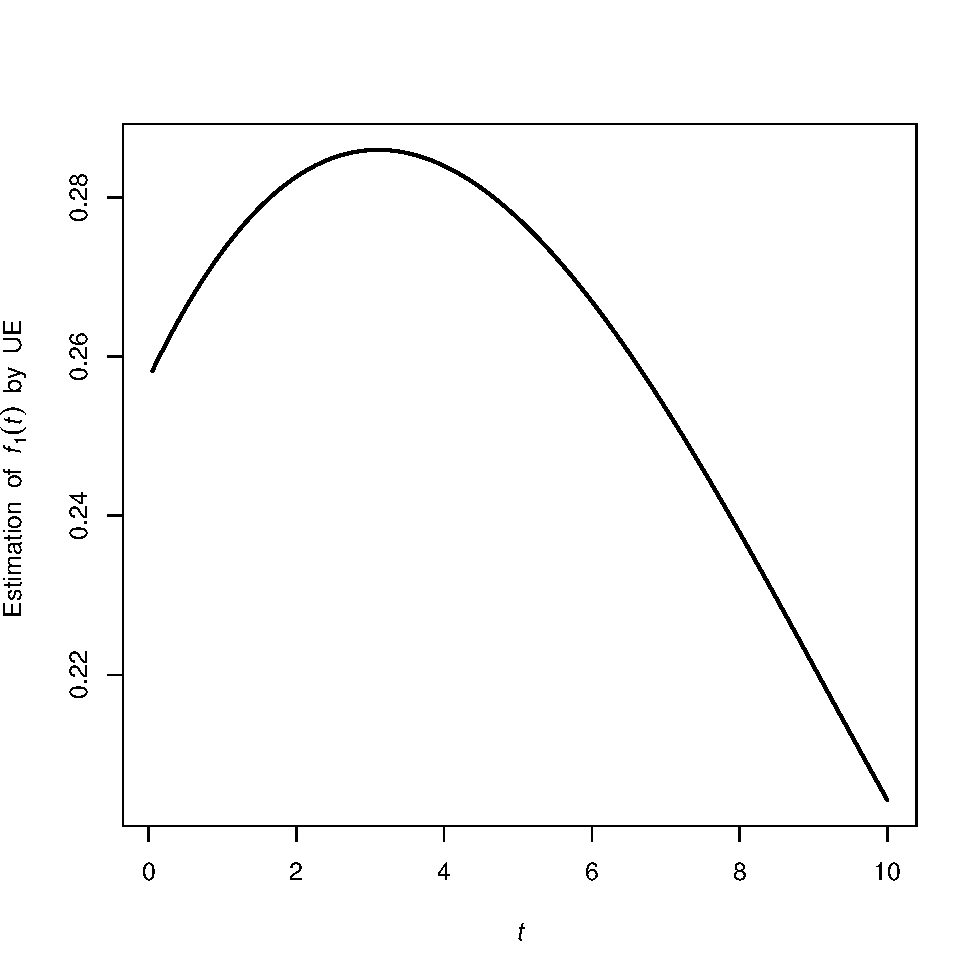
\includegraphics[scale=.15]{f1UE-eps-converted-to.pdf}&
%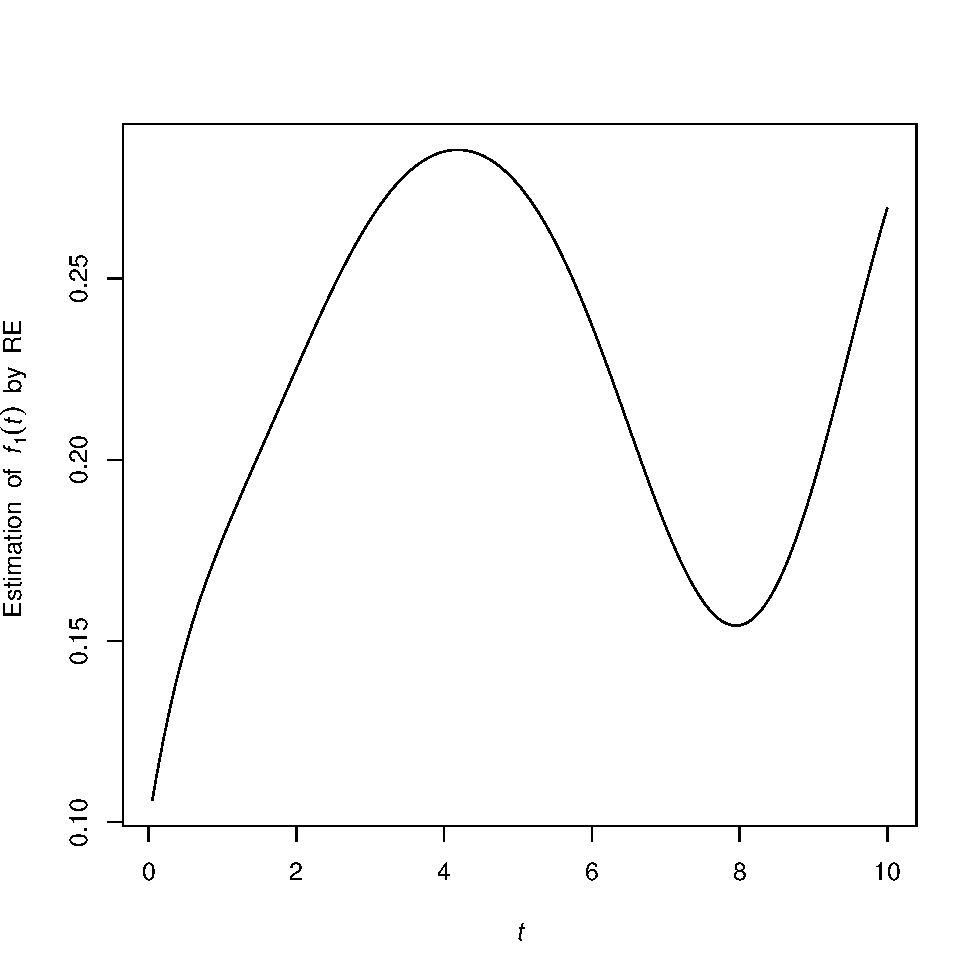
\includegraphics[scale=.15]{f1RE-eps-converted-to.pdf}&
%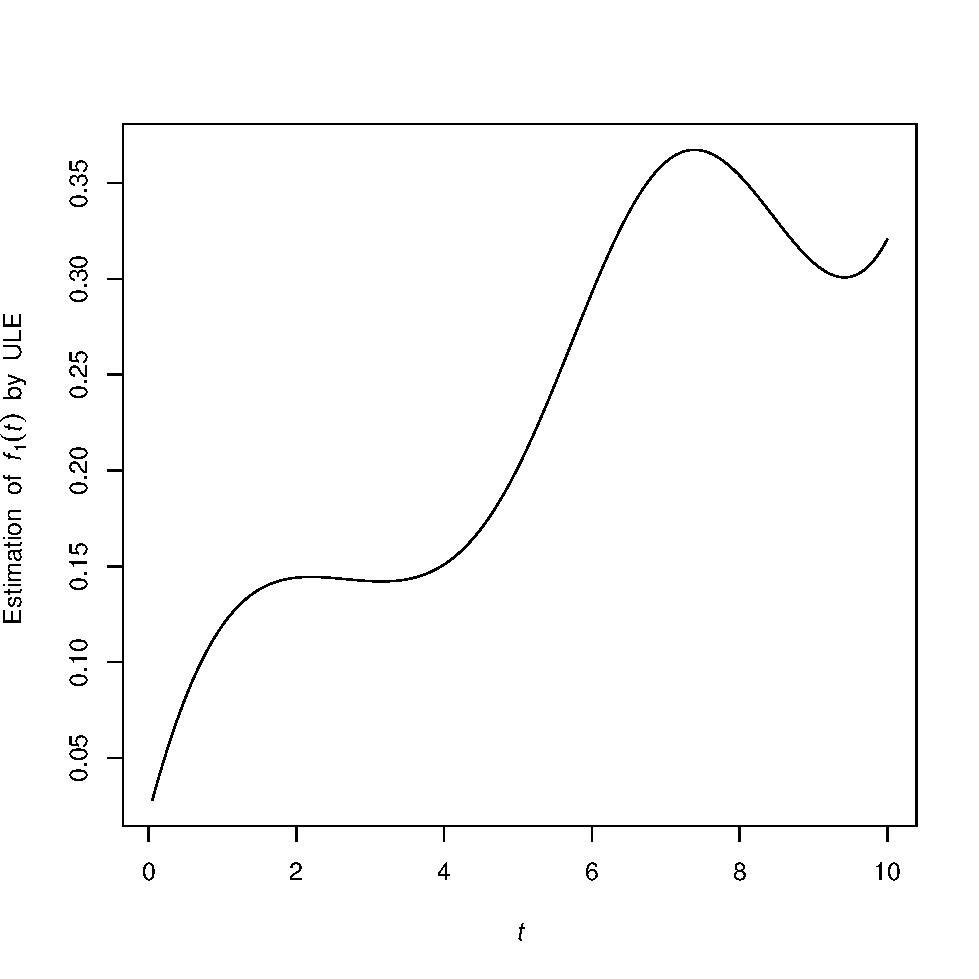
\includegraphics[scale=.15]{f1ULE-eps-converted-to.pdf}&
%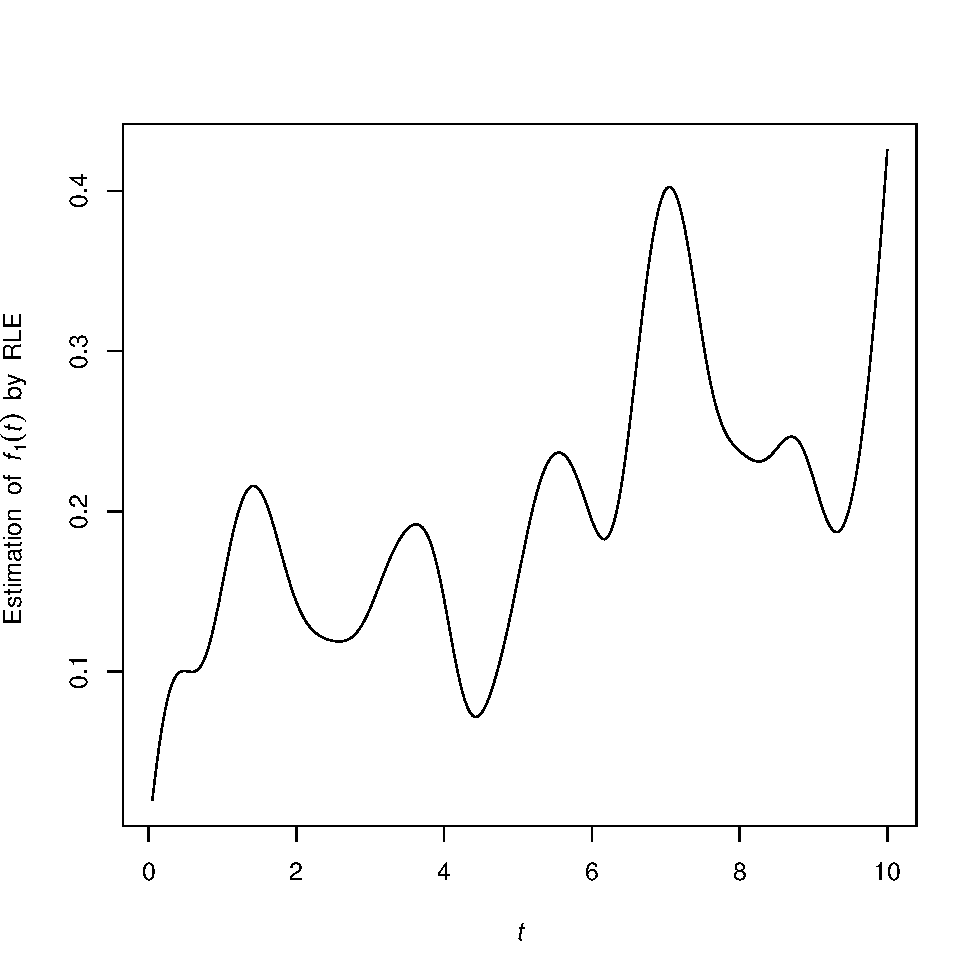
\includegraphics[scale=.15]{f1RLE-eps-converted-to.pdf}\\
%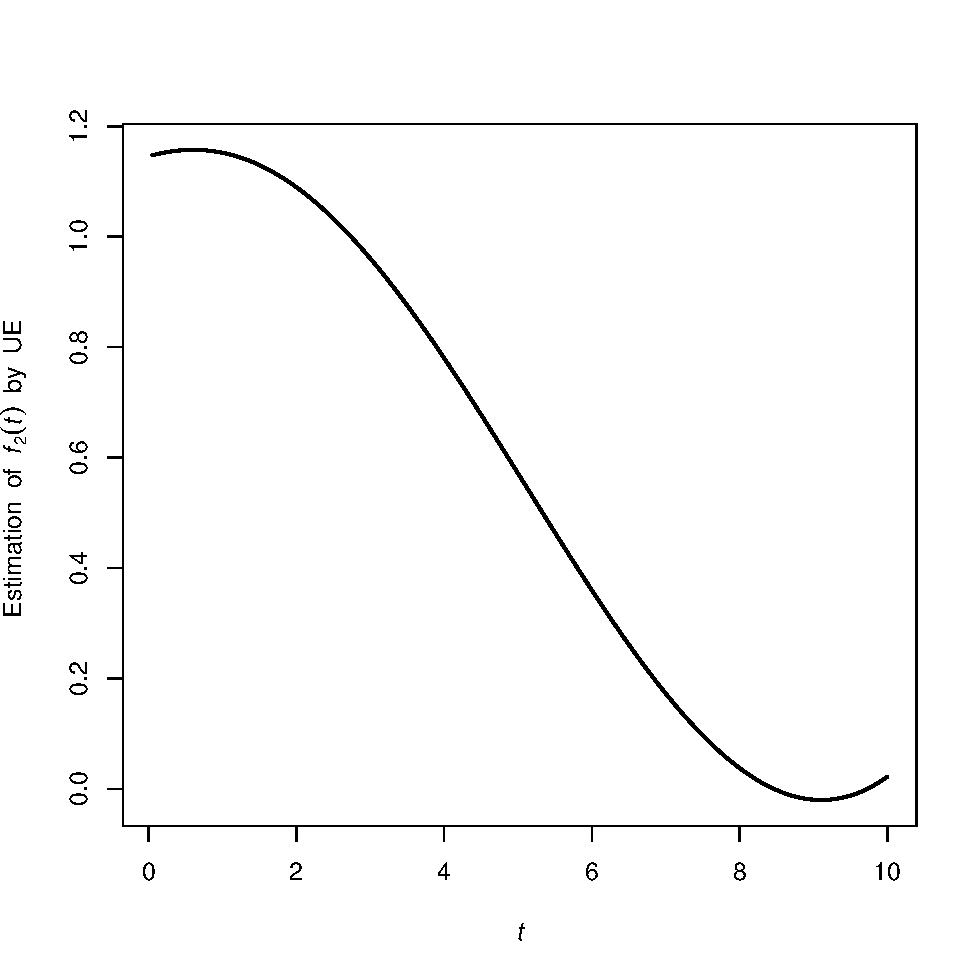
\includegraphics[scale=.15]{f2UE-eps-converted-to.pdf}&
%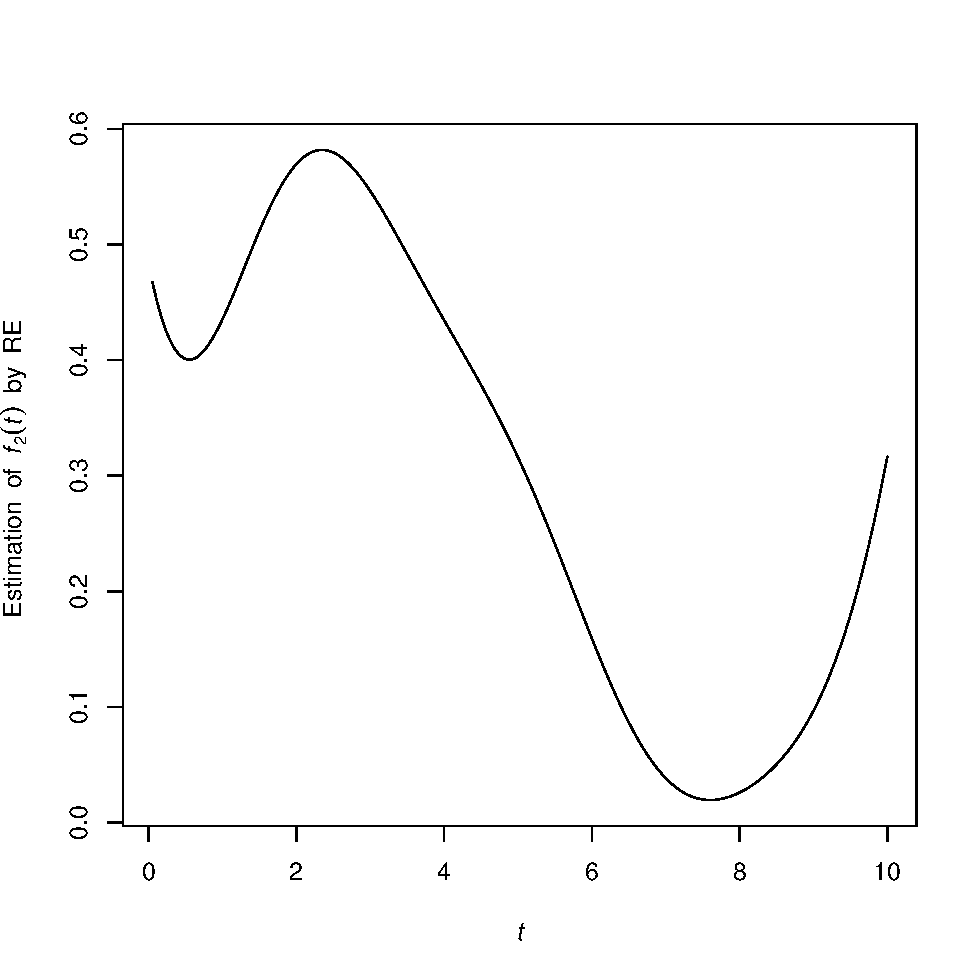
\includegraphics[scale=.15]{f2RE-eps-converted-to.pdf}&
%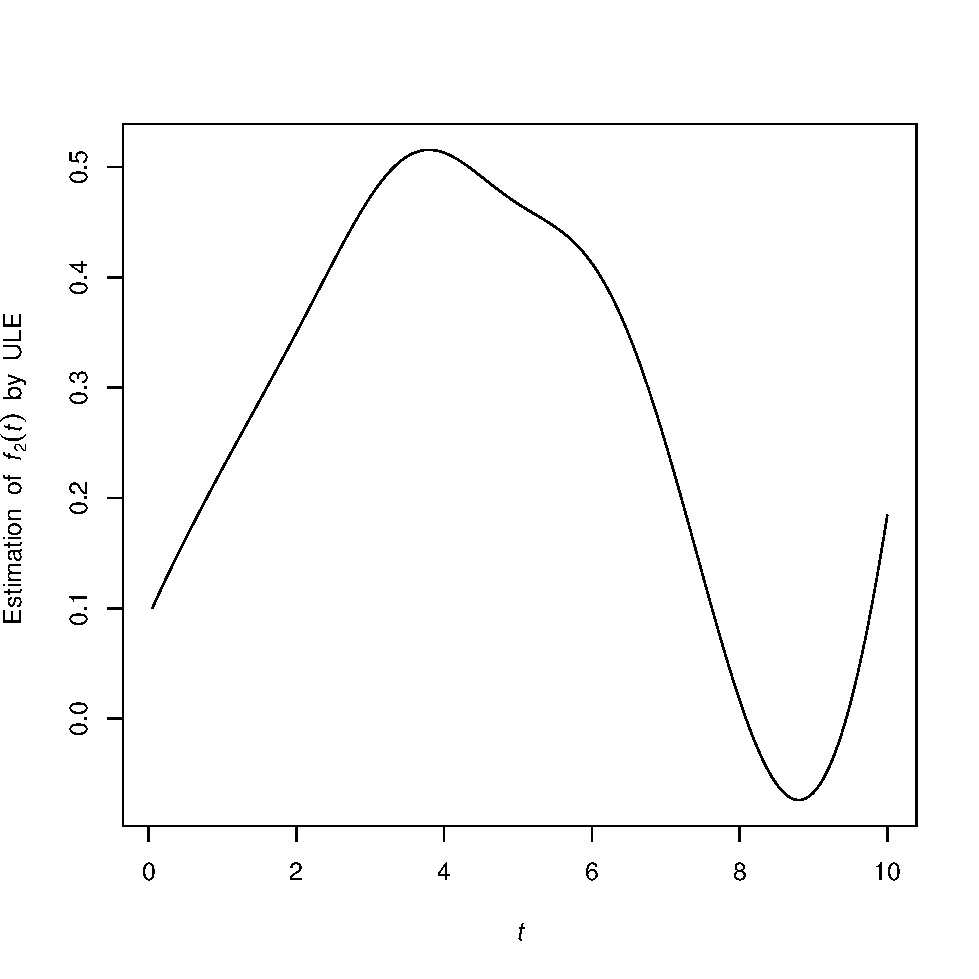
\includegraphics[scale=.15]{f2ULE-eps-converted-to.pdf}&
%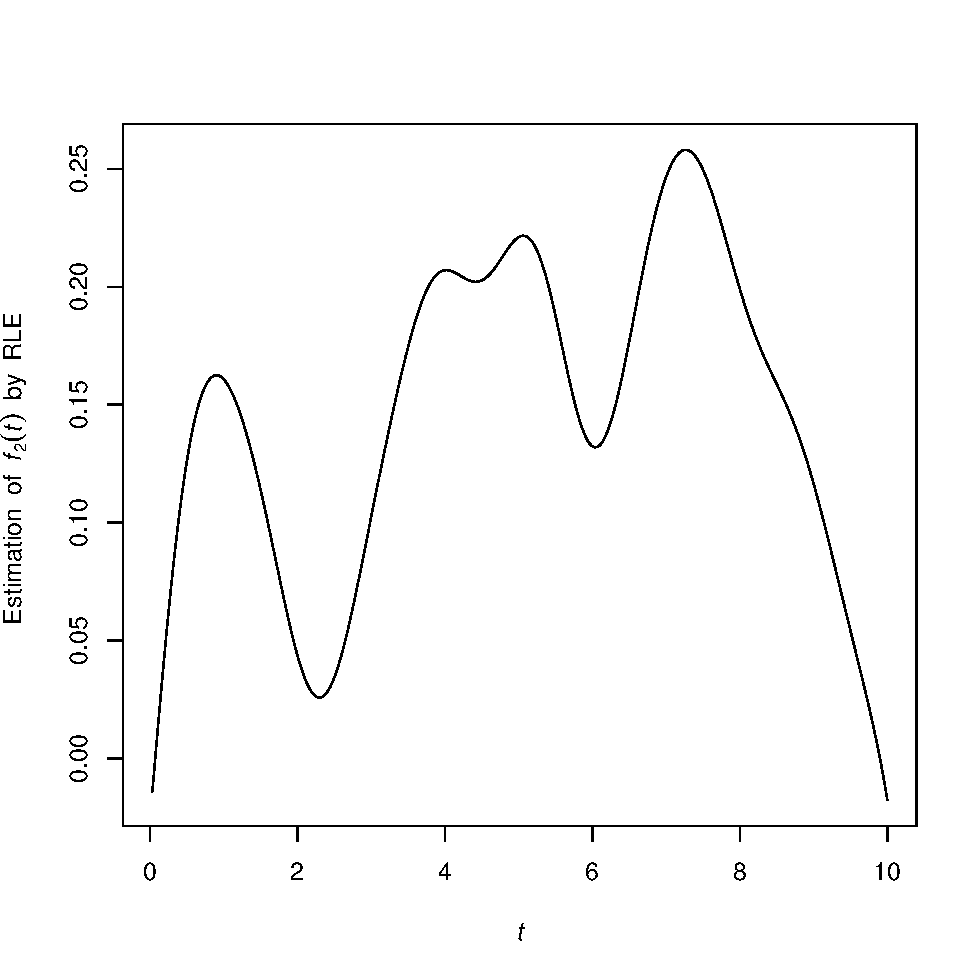
\includegraphics[scale=.15]{f2RLE-eps-converted-to.pdf}\\
%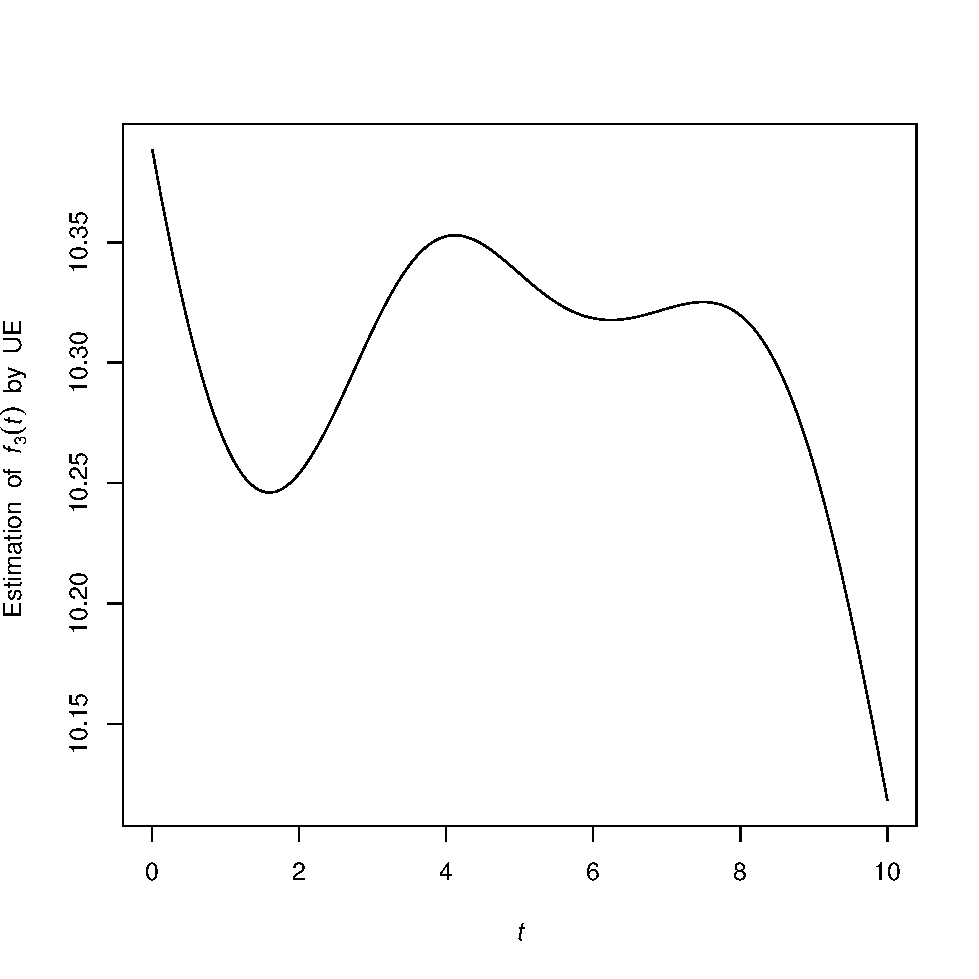
\includegraphics[scale=.15]{f3UE-eps-converted-to.pdf}&
%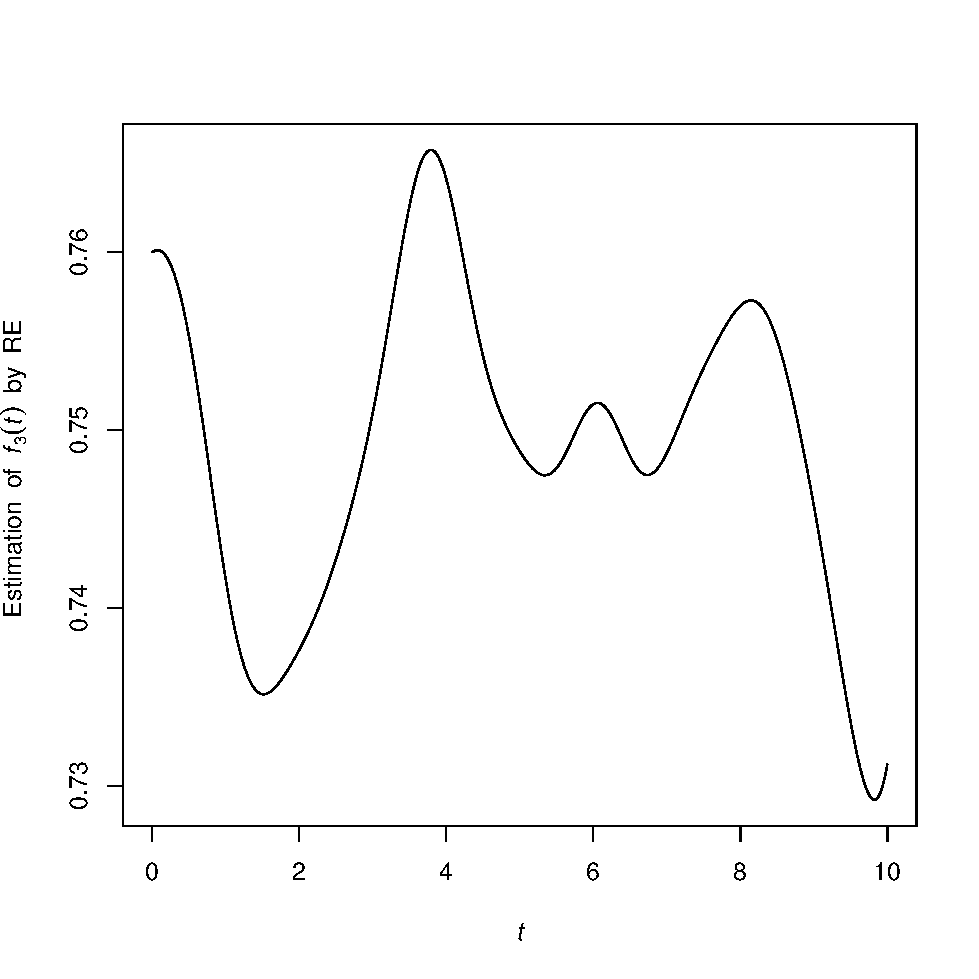
\includegraphics[scale=.15]{f3RE-eps-converted-to.pdf}&
%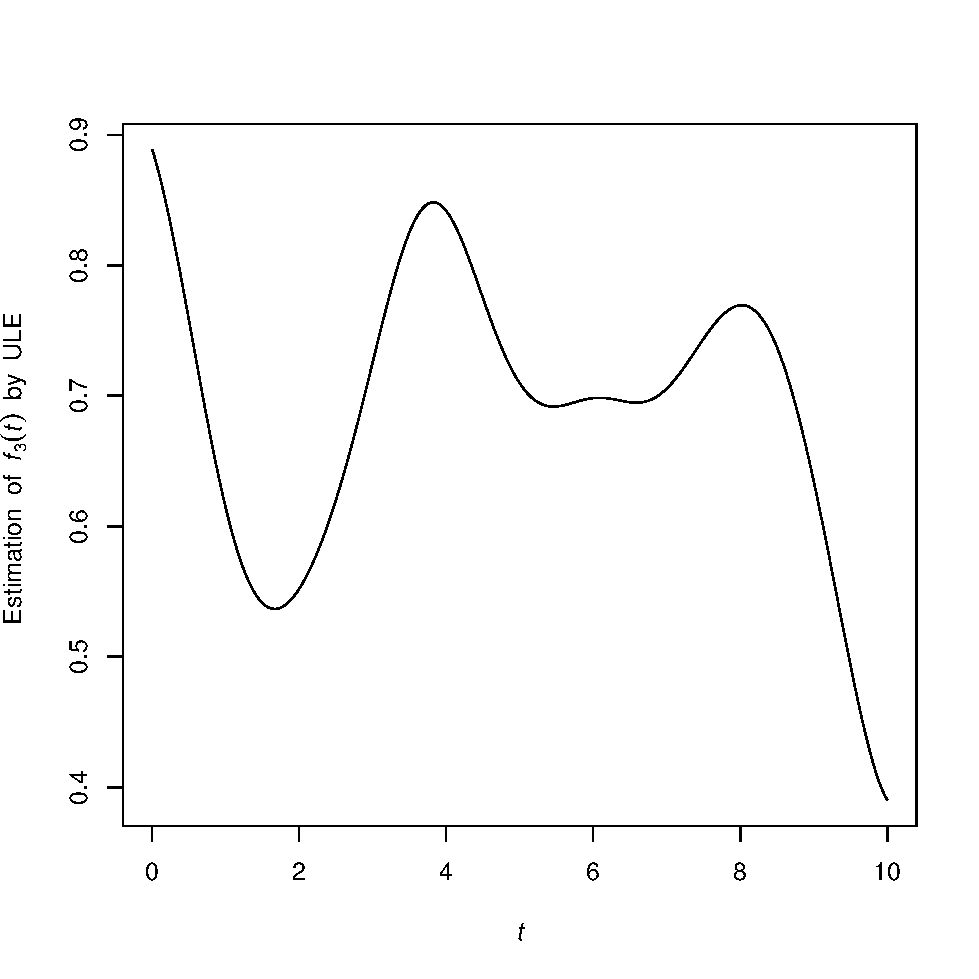
\includegraphics[scale=.15]{f3ULE-eps-converted-to.pdf}&
%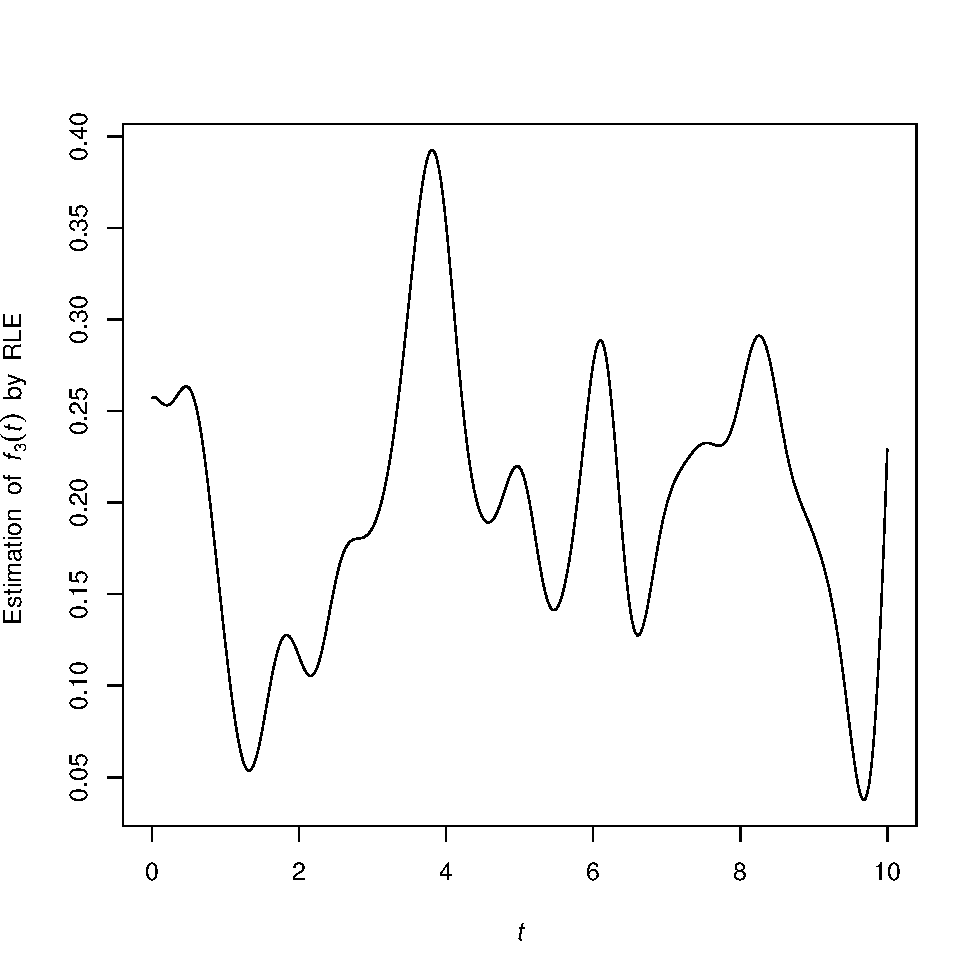
\includegraphics[scale=.15]{f3RLE-eps-converted-to.pdf}
%\end{tabular}
%\caption{\small{The estimations of the three nonparametric parts of model \eqref{eq21} for $r_x=0.99$.}}\label{fig7}
\end{figure}

Figure \ref{fig6} displays the risk functions and the corresponding $\delta$ values plotted against $d$ for the proposed estimators. To examine the isolated effect of each Liu parameter $d$, the values of $\delta$ are plotted as a function of each $d$. As can be seen from Figure \ref{fig6}, for all values of $d$, the Liu-type versions of the proposed estimators outperform their non-Liu-type counterparts whenever $\delta$ is positive. Moreover, in every case, the maximum values of $\delta$ correspond to the optimal choices of $d$, indicating the superiority of the Liu-type estimators over the non-Liu-type alternatives.

%For estimating of nonparametric part, we simulate response from model \eqref{eq21} for $T=3000$ again.
%In Figure \ref{fig7}, the nonparametric estimations of the model \eqref{eq21} for the proposed estimators are plotted. These functions are difficult to estimate and provides
%a good test for nonparametric regression methods. The
%functions are spatially inhomogeneous which means that its
%smoothness (second derivatives) varies over $t$.


\subsection{Case study}

To assess and demonstrate the benefits of applying the methods developed in this study, we employ a panel dataset that has served for many decades as a useful benchmark for evaluating multi-equation estimators and illustrating their advantages within partially linear SUR models. These data are accessible through the online supplementary materials of Greene \cite{Green2003}. The dataset includes yearly observations from 1920 to 1941 for five firms (out of the ten originally examined in the study).

\begin{table}
\centering
\caption{Evaluation of estimators at optimum values of $d$ for model \eqref{real2} based on the real data set (transposed)} \label{tab:33}
\small
\begin{tabular}{lcccccccc}
\hline
Equation & Method & $\hat{\beta}_0$ & $\hat{\beta}_1$ & $\hat{\beta}_2$ & $\hat{\beta}_3$ & $d_{opt}$ & ${\rm GCV}(\hat\beta;\beta)$ \\
\hline
Eq. 1 & UE  & -0.09 & 0.15 & 0.81 & - & - & 1.46 \\
                       & RE  & -0.09 & 0.15 & 0.80 & - & - & 0.53 \\
                       & ULE & -0.07 & 0.15 & 0.81 & - & 0.22 & 1.13 \\
                       & RLE & -0.06 & 0.15 & 0.80 & - & 0.30 & 0.46 \\
\hline
Eq. 2 & UE  & 10.34 & 0.48 & 0.33 & -0.11 & - & 1.46 \\
                       & RE  & 9.96 & 0.49 & 0.33 & -0.11 & - & 0.53 \\
                       & ULE & 9.47 & 0.48 & 0.32 & -0.11 & 0.22 & 1.13 \\
                       & RLE & 9.88 & 0.50 & 0.33 & -0.11 & 0.30 & 0.46 \\
\hline
Eq. 3 & UE  & 1.88 & 0.43 & 0.15 & 0.14 & - & 1.46 \\
                       & RE  & 0.31 & 0.42 & 0.18 & 0.15 & - & 0.53 \\
                       & ULE & 1.80 & 0.43 & 0.10 & 0.14 & 0.22 & 1.13 \\
                       & RLE & 1.77 & 0.41 & 0.18 & 0.14 & 0.30 & 0.46 \\
\hline
\end{tabular}
\end{table}

We begin by applying the SUR model to analyze the data, where the following variables are considered: consumption ($consump$), corporate profits ($corpProf$), corporate profits from the previous year ($corpProfLag$), the sum of private and government wage bills ($wages$), investment ($invest$), capital stock from the previous year ($capitalLag$), the private wage bill ($privWage$), gross national product ($gnp$), gross national product from the previous year ($gnpLag$), and a time trend measured as years since 1931 ($trend$). Accordingly, the adequacy of the subsequent SUR model is assessed through its fit to the aforementioned dataset. The partially linear SUR model is specified as follows:
\begin{eqnarray}\label{real2}
&&\hspace{-1cm}Eq.1\quad consump_{i}=\beta_{0}+\beta_{1}(corpProf)_{i}+\beta_{2}(wages)_{i}+f((corpProfLag)_{i}),~ i=1,\ldots,20,\nonumber\\
&&\hspace{-1cm}Eq.2\quad invest_{i}=\beta_{0}+\beta_{1}(corpProf)_{i}+\beta_{2}(corpProfLag)_{i}+\beta_{3}(capitalLag)_{i},~ i=1,\ldots,20,\nonumber\\
&&\hspace{-1cm}Eq.3\quad privWage_{i}=\beta_{0}+\beta_{1}(gnp)_{i}+\beta_{2}(gnpLag)_{i}+\beta_{3}(trend)_{i},~ i=1,\ldots,20.
\end{eqnarray}

In this study, we employ generalized cross-validation (GCV) to determine the optimal value of the Liu parameter, as well as to assess the proposed estimator using a metric other than the mean squared error, thereby helping to avoid overfitting when predicting real data. The GCV criterion serves as an observable and efficient proxy for the risk function, implying that minimizing GCV is equivalent to minimizing the risk. This estimator represents a rotation-invariant version of Allen's PRESS, also known as standard cross-validation. It functions similarly to a risk improvement estimator but does not require an estimate of the error variance $\sigma^2$. Owing to these advantageous properties, GCV is used to select the optimum Liu parameter (for further details, see \cite{Amini2015}). Following the results of \cite{Roozbeh2018}, the GCV criterion for the proposed methods can be computed as follows:
\begin{eqnarray*}\label{gcv0}
{\rm GCV}(\hat{\boldsymbol\beta}_j;\boldsymbol\beta)=\frac{\frac{1}{n}\big({\widetilde{\boldsymbol{Y}}}-
\hat{\widetilde{\boldsymbol{Y}}}_j\big)^\top\big({\widetilde{\boldsymbol{Y}}}-\hat{\widetilde{\boldsymbol{Y}}}_j\big)}{\Big(1-\frac{1}{n}{\rm tr}\big(\boldsymbol L(\hat{\boldsymbol\beta}_j\big)\Big)^2},\quad j=1,\ldots,10,
\end{eqnarray*}
where $\hat{\widetilde{\boldsymbol{Y}}}_j=\boldsymbol L(\hat{\boldsymbol\beta}_j){\widetilde{\boldsymbol{Y}}}$ in which $\boldsymbol L(\hat{\boldsymbol\beta}_j)$ is the hat matrix of $j$th approach.

Based on the results presented in Table \ref{tab:33}, it can be inferred that the PRLE performs with notable accuracy in estimating both the linear and non-linear components relative to the alternative methods.


\begin{thebibliography}{1}
	
\bibitem{Akdeniz1995}
Akdeniz, F. \& Kaciranlar, S., (1995). On the almost unbiased generalized Liu estimator and unbiased estimation of the bias and MSE, Comm. Statist. Theo. Meth. , 24: 1789-1797.

%\bibitem{Algamal2025}
%Algamal, Z.Y. (2025). A modified ridge estimator in Cox regression model. Communications in Statistics - Simulation and Computation{\color{black}, 1-8.}
\bibitem{Algamal2022}
Algamal, Z.Y. \& Abonazel, M.R. (2022). Developing a Liu-type estimator in beta regression model. Concurrency and Computation: Practice and Experience. 34(5), e6685.

\bibitem{Algamal2018}
Algamal, Z.Y., \& Asar, Y. (2018). Liu-type estimator for the gamma regression model. Communications in Statistics - Simulation and Computation, 49, 2035 - 2048.

\bibitem{Amin2021}
Amin, M., Akram, M.N., \& Kibria, B.M. (2021). A new adjusted Liu estimator for the Poisson regression model. Concurrency Comp. Pract. Exper., {\color{black}33(20), e6340.}

\bibitem{Amini2015}
Amini, M., \& Roozbeh, M. (2015). Optimal partial ridge estimation in restricted semiparametric regression models. J. Multivar. Anal., 136, {\color{black}26 - 40.}

%\bibitem{Carriero2015}
%Carriero, A., Clark, T. E., \& Marcellino, M. (2015). Bayesian VARs: Specification choices and forecast accuracy. J. Appl. Econometrics, 30(1), 46 - 73.

\bibitem{Forzani2021}
Forzani, L., \& Su, Z. (2021). Envelopes for elliptical multivariate linear regression. Statist. Sinica, 31(1), 301 - 332.

\bibitem{Galea2000}
Galea, M., Marco, R., \& Gilberto, A.P. (2000). Diagnostic Methods in Elliptical Linear Regression Models. Brazilian J. Prob. Statist., 14, 167 - 84.

%\bibitem{Green2003}
%Greene, W.H. (2003). Econometric Analysis. 5th edition. Prentice Hall, USA.

%\bibitem{Korobilis2013}
%Korobilis, D. (2013). VAR forecasting using Bayesian variable selection. J. Appl. Econometric Meth., 18(2), 237 - 258.
		
\bibitem{Liu1993}
Liu, K., (1993). A new class of biased estimate in linear regression. Comm. Statist. Theo. Meth., 22, 393 - 402.

\bibitem{Liu2014}
Liu, L., \& Wang, L. (2014). A new Liu-type estimator in SUR models. Comm. Statist. Theo. Meth., 43(19), 4135 - 4145.

\bibitem{Månsson2013}
Månsson, K. (2013). Developing a Liu estimator for the negative binomial regression model: method and application. J. Statist. Comp. Simu., 83(9), 1773 - 1780.

\bibitem{Månsson2012-2}
Månsson, K., Kibria, B.M., Sjölander, P., \& Shukur, G. (2012). Improved Liu Estimators for the Poisson Regression Model. Int. J. Statist. Prob., 1, 2 - 6.

\bibitem{Månsson2012-3}
Månsson, K., Kibria, B.M., \& Shukur, G. (2012). On Liu Estimators for the Logit Regression Model. Economic Modelling, 29, 1483 - 1488.

\bibitem{Roozbeh2018} 
Roozbeh, M. (2018) {Optimal QR-based estimation in partially linear regression models with correlated errors using GCV criterion.} {Computational Statistics \& Data Analysis}, 117, 45-61.

\bibitem{Roozbeh2012}
Roozbeh, M., Arashi, M., \& Gasparini, M. (2012) Seemingly unrelated ridge regression in Semiparametric Models, Comm. Statist. Theo. Meth., 41, 1364 - 1386.

\bibitem{Srivastava2010}
Srivastava, M. S., \& Kubokawa, T. (2010). Estimation of the precision matrix of a singular Wishart distribution and its application in SUR models. J. Mult. Anal., 101(7), 1465-1478.
		
%\bibitem{Qasim2021}
%Qasim, M. et al. (2021). A new class of efficient and debiased two-step shrinkage estimators: method and application. J. Appl. Statistics, 49(16), 4181 - 4205.

\bibitem{Qasim2020}
Qasim, M., Amin, M., \& Omer, T. (2020). Performance of some new Liu parameters for the linear regression model. Comm. Statist. Theo. Meth., 49, 4178 - 4196.

\bibitem{Qasim2019}
Qasim, M., Kibria, B.M., Månsson, K., \& Sjölander, P. (2019). A new Poisson Liu Regression Estimator: method and application. J. Appl. Statist., 47, 2258 - 2271.
		
%\bibitem{Saleh2019}
%Saleh, A. K. Md. E., Arashi, M., \& Kibria, B. M. G. (2019) Theory of Ridge Regression Estimation with Applications, Wiley, USA.
		
\bibitem{Saleh2022}
Saleh, A. K. Md. E., Arashi, M., Saleh, R. A. \& Norouzirad, M. (2022) Rank-Based Methods for Shrinkage and Selection: With Application to Machine Learning, Wiley, USA.

%\bibitem{Seifollahi2025}
%Seifollahi, S., Bevrani, H. \& Algamal, Z.Y. (2025). Shrinkage Estimators in Zero-Inflated Bell Regression Model with Application. J. Statist. Theo. Pract. 19, 1.

%\bibitem{Seifollahi2024}
%Seifollahi, S., Bevrani, H., \& Algamal, Z.Y. (2024). Improved estimators in bell regression model with application. J. Statist. Comp. Sim., 94, 2710 - 2726.

%\bibitem{Seifollahi2024-2}
%Seifollahi, S., Bevrani, H., \& Månsson, K. (2024). Bayesian Analysis of the Beta Regression Model Subject to Linear Inequality Restrictions with Application. arXiv preprint arXiv:2401.13787.

%\bibitem{Seifollahi2023}
%Seifollahi, S., \& Bevrani, H., (2023) James-Stein type estimators in beta regression model: simulation and application. Hacettepe J. Math. Statist. 52(4), {\color{black}1046 - 1065.}

%\bibitem{sh09}  
%Sheather, S.J., (2009) {A Modern Approach to Regression with R}, Springer, New York.
	
\bibitem{Speckman1988}
Speckman, P., (1988).  Kernel smoothing in partial linear
models. J. Royal Statist. Soc.: Ser. B, 50, 413 - 437.
		

\bibitem{Zellner1962}
Zellner, A., (1962). An efficient method of estimating
seemingly unrelated regressions and tests for aggregation bias.
J. Amer. Statist. Assoc., 57, 348 - 368.


\end{thebibliography}

\end{document}





	
Akdeniz, F. & Kaciranlar, S., (1995). On the almost unbiased generalized Liu estimator and unbiased estimation of the bias and MSE, Comm. Statist. Theo. Meth. , 24: 1789-1797.

Algamal, Z.Y. & Abonazel, M.R. (2022). Developing a Liu-type estimator in beta regression model. Concurrency and Computation: Practice and Experience. 34(5), e6685.

Algamal, Z.Y., & Asar, Y. (2018). Liu-type estimator for the gamma regression model. Communications in Statistics - Simulation and Computation, 49, 2035 - 2048.

Amin, M., Akram, M.N., & Kibria, B.M. (2021). A new adjusted Liu estimator for the Poisson regression model. Concurrency Comp. Pract. Exper., 33(20), e6340.

Amini, M., & Roozbeh, M. (2015). Optimal partial ridge estimation in restricted semiparametric regression models. J. Multivar. Anal., 136, 26 - 40.

Forzani, L., & Su, Z. (2021). Envelopes for elliptical multivariate linear regression. Statist. Sinica, 31(1), 301 - 332.

Galea, M., Marco, R., & Gilberto, A.P. (2000). Diagnostic Methods in Elliptical Linear Regression Models. Brazilian J. Prob. Statist., 14, 167 - 84.

Liu, K., (1993). A new class of biased estimate in linear regression. Comm. Statist. Theo. Meth., 22, 393 - 402.

Liu, L., & Wang, L. (2014). A new Liu-type estimator in SUR models. Comm. Statist. Theo. Meth., 43(19), 4135 - 4145.

Månsson, K. (2013). Developing a Liu estimator for the negative binomial regression model: method and application. J. Statist. Comp. Simu., 83(9), 1773 - 1780.

Månsson, K., Kibria, B.M., Sjölander, P., & Shukur, G. (2012). Improved Liu Estimators for the Poisson Regression Model. Int. J. Statist. Prob., 1, 2 - 6.

Månsson, K., Kibria, B.M., & Shukur, G. (2012). On Liu Estimators for the Logit Regression Model. Economic Modelling, 29, 1483 - 1488.

Roozbeh, M. (2018) Optimal QR-based estimation in partially linear regression models with correlated errors using GCV criterion. Computational Statistics & Data Analysis, 117, 45-61.

Roozbeh, M., Arashi, M., & Gasparini, M. (2012) Seemingly unrelated ridge regression in Semiparametric Models, Comm. Statist. Theo. Meth., 41, 1364 - 1386.

Srivastava, M. S., & Kubokawa, T. (2010). Estimation of the precision matrix of a singular Wishart distribution and its application in SUR models. J. Mult. Anal., 101(7), 1465-1478.
		
Qasim, M., Amin, M., & Omer, T. (2020). Performance of some new Liu parameters for the linear regression model. Comm. Statist. Theo. Meth., 49, 4178 - 4196.

Qasim, M., Kibria, B.M., Månsson, K., & Sjölander, P. (2019). A new Poisson Liu Regression Estimator: method and application. J. Appl. Statist., 47, 2258 - 2271.
		
Saleh, A. K. Md. E., Arashi, M., Saleh, R. A. & Norouzirad, M. (2022) Rank-Based Methods for Shrinkage and Selection: With Application to Machine Learning, Wiley, USA.

Speckman, P., (1988).  Kernel smoothing in partial linear models. J. Royal Statist. Soc.: Ser. B, 50, 413 - 437.
		

Zellner, A., (1962). An efficient method of estimating seemingly unrelated regressions and tests for aggregation bias. J. Amer. Statist. Assoc., 57, 348 - 368.


